\section{Merge-Sort}

\textbf{Merge-Sort} ist ein \textbf{stabiler}, auf Schlüsselvergleichen basierender Sortieralgorithmus, der \textbf{nicht in place} sortiert.

\subsection{Methode}

\textbf{Merge-Sort} nutzt \textbf{divide-and-conquer}, um ein Feld zu sortieren.\\
Die wesentliche Arbeit erfolgt hier in den Merge-Schritten, im Gegensatz zu \textbf{Quicksort}, bei dem die eigentliche Arbeit im Partitionierungs-Schritt stattfindet (vgl.~\cite[174]{GD18e}).\\
I.d.R. benötigt Merge-Sort linear viel zusätzlichen Speicherplatz (vgl.~\cite[112]{OW17b}.

\noindent
Der Algorithmus teilt die Eingabefolge rekursiv in zwei gleich-große Folgen auf, bis $n$ ein-elementige Folgen vorhanden sind (eine ein-elementige Menge gilt als sortiert).\\
Im Anschluss werden die Folgen miteinander verschmolzen, und zwar so, dass die miteinander verschmolzenen Folgen immer in sortierter Reihenfolge vorliegen.\\
Das ganze wird so lange wiederholt, bis die Folge mit $n$ Elementen wieder rekonstruiert ist: Sie liegt dann in sortierter Reihenfolge vor (s. Abbildung~\ref{fig:mergesort}).\\


\subsection{Implementierung}

Das folgende Beispiel beinhaltet nicht die Methoden für die Partitionierung und das Verschmelzen.

\begin{minted}{java}
    mergeSort(int[] arr, int start, int end) {
        if (arr.length == 1) {
            return arr;
        }

        int mid = (start + end) / 2;
        int[] left = divide(arr, start, mid);
        int[] right = divide(arr, mid + 1, end);

        left = mergeSort(left, 0, left.length - 1);
        right = mergeSort(right, 0, right.length - 1);

        arr = merge(arr, left, right, start);

        return arr;
    }
\end{minted}

\begin{figure}
    \begin{center}
        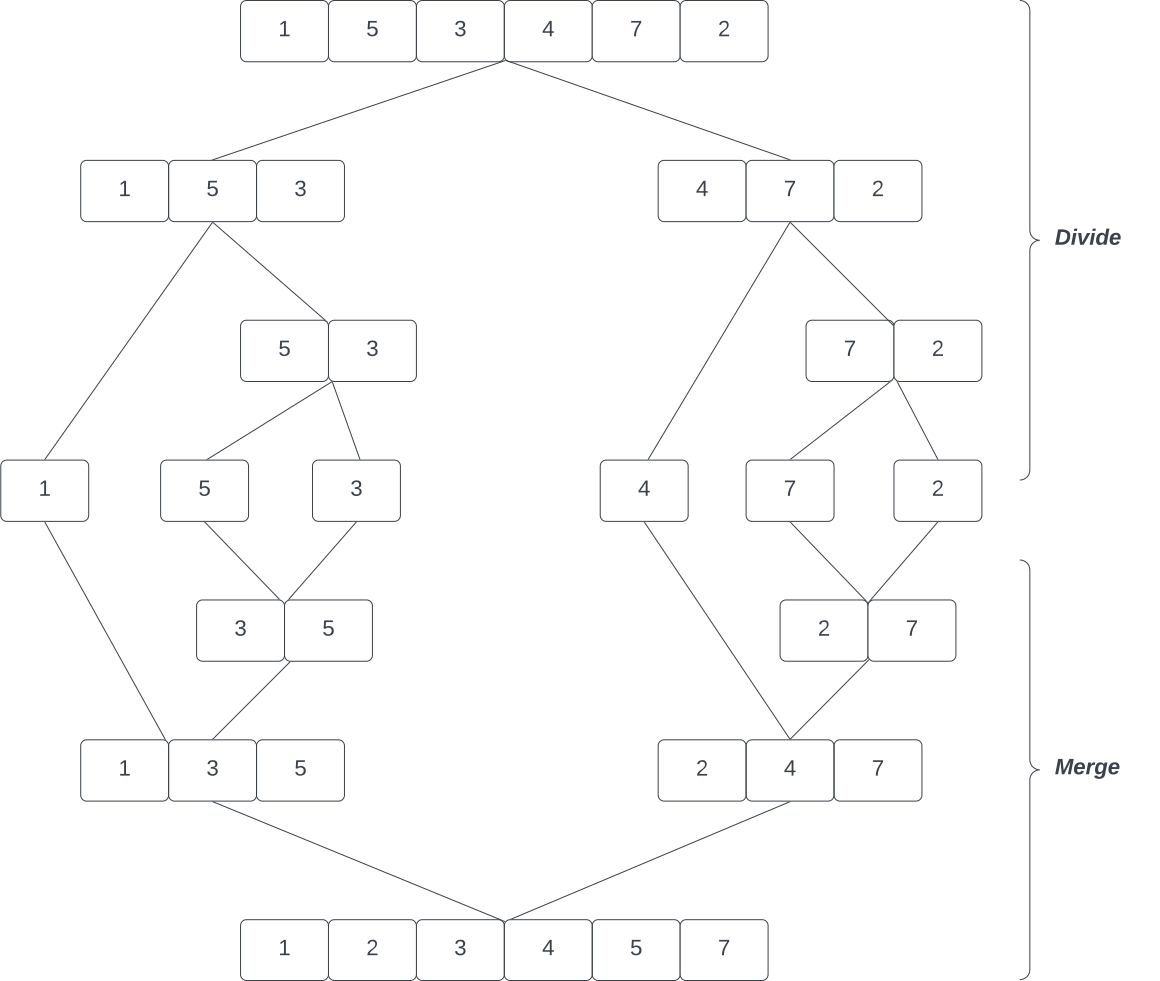
\includegraphics[scale=0.3]{chapters/Sortierverfahren/img/mergesort}
        \caption{Anwendung von Merge-Sort auf das Feld $1,\ 5,\ 3,\ 4,\ 7,\ 2$.  (Quelle: eigene)}
        \label{fig:mergesort}
    \end{center}
\end{figure}


\subsection{Laufzeit}

\begin{itemize}
    \item \textbf{worst-case}: Merge-Sort hat eine Laufzeit von $O(n\ log\ n)$.\\
        Das Aufteilen des Feldes benötigt $O(log\ n)$, in jedem Schritt werden Operationen mit $O(n)$ Zeit durchgeführt (aufteilen  oder verschmelzen) \footnote{
        Das Verschmelzen von zwei Teilfeldern erfolgt durch paralleles Durchlaufen mti anschliessendem Einfügen in ein sortiertes Teilfeld, wozu $O(n)$ Zeit benötigt wird (vgl. Skript (Teil 2) ``7.4.1 MergeSort``).
    }
    \item \textbf{average-case}: $O(n\ log\ n)$
    \item \textbf{best-case}: $O(n\ log\ n)$
\end{itemize}

\begin{tcolorbox}
    Die Rekursionstiefe ist bei \textbf{Merge-Sort} logarithmisch beschränkt (mit $\lceil log\ n \rceil$), im Gegensatz zu \textbf{Quicksort} (vgl.~\cite[116]{OW17b}).
\end{tcolorbox}